\documentclass{article}
\bibliographystyle{plain}
\usepackage{natbib}
\usepackage{bibentry}
\usepackage{graphicx}
\usepackage{placeins}
\usepackage[svgnames]{xcolor} % Dartmouth green
\definecolor{dartmouthgreen}{HTML}{017d39}
\definecolor{linkblue}{HTML}{0022f0}
\usepackage[colorlinks=true,allcolors=linkblue]{hyperref}
\setlength\topmargin{0pt}
\addtolength\topmargin{-\headheight}
\addtolength\topmargin{-\headsep}
\setlength\oddsidemargin{0pt}
\setlength\textwidth{\paperwidth}
\addtolength\textwidth{-2in}
\setlength\textheight{\paperheight}
\addtolength\textheight{-2in}
\usepackage{layout}

\nobibliography*

\title{\vspace{-2.5cm} Analysis of Data From 'Large-Scale Multi-omic Analysis of COVID-19 Severity', Overmyer et al. 2021}

\author{
QBS 103 Final Project\\
Project Author: Sabin Hart\\
Contact: sabin.d.hart.gr@dartmouth.edu\\}
\date{}

\begin{document}
\maketitle

\textbf{\textit{Abstract}---
This study performs a detailed analysis of data from Overmyer et al.'s 2021 "Large-scale multi-omic analysis of COVID-19 severity," focusing on the gene ABCA7. Using R, the study explores the relationship between ABCA7 expression and COVID-19 severity, ICU status, and demographic factors. Key findings include a negative correlation between ABCA7 expression and disease severity, variations in expression across sex and ICU status, and the importance of normalization in visualizing gene expression patterns. Summary statistics and visualizations are provided to support these findings.}

\subsection*{1. Introduction}

The body of this study is built off the data and analysis of "Large-scale
multi-omic analysis of COVID-19 severity" (2021) by Overmyer et al \cite{Overmyer2021}. The authors map 128 COVID-19 positive and negative blood samples with genotypical features, disease severity and symptomality. These data include the expression of nearly 100 genes as well as ICU status, some demographic features, and evaluative scores.

I focus my analysis primarily on the gene ABCA7. According to the National Institute of Health, ABCA7 is a member of the ABC1 subfamily of ATP-binding casette transporters, the only subfamily found exclusively in multicellular eukaryotes. Its exact function is not yet known  "...however, the expression pattern suggests a role in lipid homeostasis in cells of the immune system. \cite{nihABCA7Binding}


\subsection*{2. Data and Methods}

The data were collected, cleaned, and prepared using R Version 4.0.4. In addition to the Base R functionality, the following packages were used: tidyverse - for a variety of data processing and visualization techniques \cite{R-tidyverse}; pheatmap - for visualizing the heatmaps \cite{R-pheatmap}; ggthemes - for additional data visualization themes \cite{R-ggthemes}; stringr - for better string operations \cite{R-stringr}; rlist - for better list operations \cite{R-rlist}; and stargazer - for outputting R data in LaTeX tables \cite{R-stargazer}.

The data were provided in two parts: a gene expression chart and a phenotype information chart. By transposing and joining based on the participants' IDs, an overall data table was created.

With the data, I create a histogram, which displays the distribution of ABCA7 expression. I also create a scatter plot between ABCA7 and disease severity, with a smoothed linear regression, and a boxplot showing the gene's association with sex and ICU status.

In addition, I plot heatmaps of a subset of 15 genes against 15 participants with highest variance. Clustering is performed to better display results, using euclidean distance, or the square root of the sum of squared distances as the clustering value. Since these are genes and absolute expression can vary heavily, I present both a crude and a normalized heatmap. The normalization is such that the mean expression is zero and standard deviation is one.

The final plot is a density plot of the expression of a subset of 5 of the genes chosen for the heatmap. This shows their relative densities at different levels of expression. These plots are all displayed in Section 3.

With the data complete, the summary statistics are displayed in Table \ref{Table 1}. Stratified by sex, results for the continuous variables (Age, Apache II Score, and Ferritin) are displayed as 'mean (standard deviation)' while discrete variables (On Mechanical Ventilation and In ICU) are displayed with 'count (percent\%)'.

\begin{table}[!htbp] \centering 
  \caption{Summary Statistics} 
  \label{Table 1} 
\begin{tabular}{@{\extracolsep{5pt}} cccccccc} 
\\[-1.8ex]\hline 
\hline \\[-1.8ex] 
Sex & Age & Apache II & Ferritin (ng/mL) & Mechanical Ventilation & In ICU & Count \\ 
\hline \\[-1.8ex] 
Female & 66.5 (16.2) & 21.4 (8.9) & 668 (1087) & 16 (31.4\%) & 24 (47.1\%) & 51 \\ 
Male & 62.3 (12.1) & 20.7 (7.5) & 1073 (911) & 35 (47.3\%) & 41 (55.4\%) & 74 \\ 
\hline \\[-1.8ex] 
\end{tabular} 
\end{table} 

\subsection*{3. Results}


\begin{figure}[h!]
    \centering
    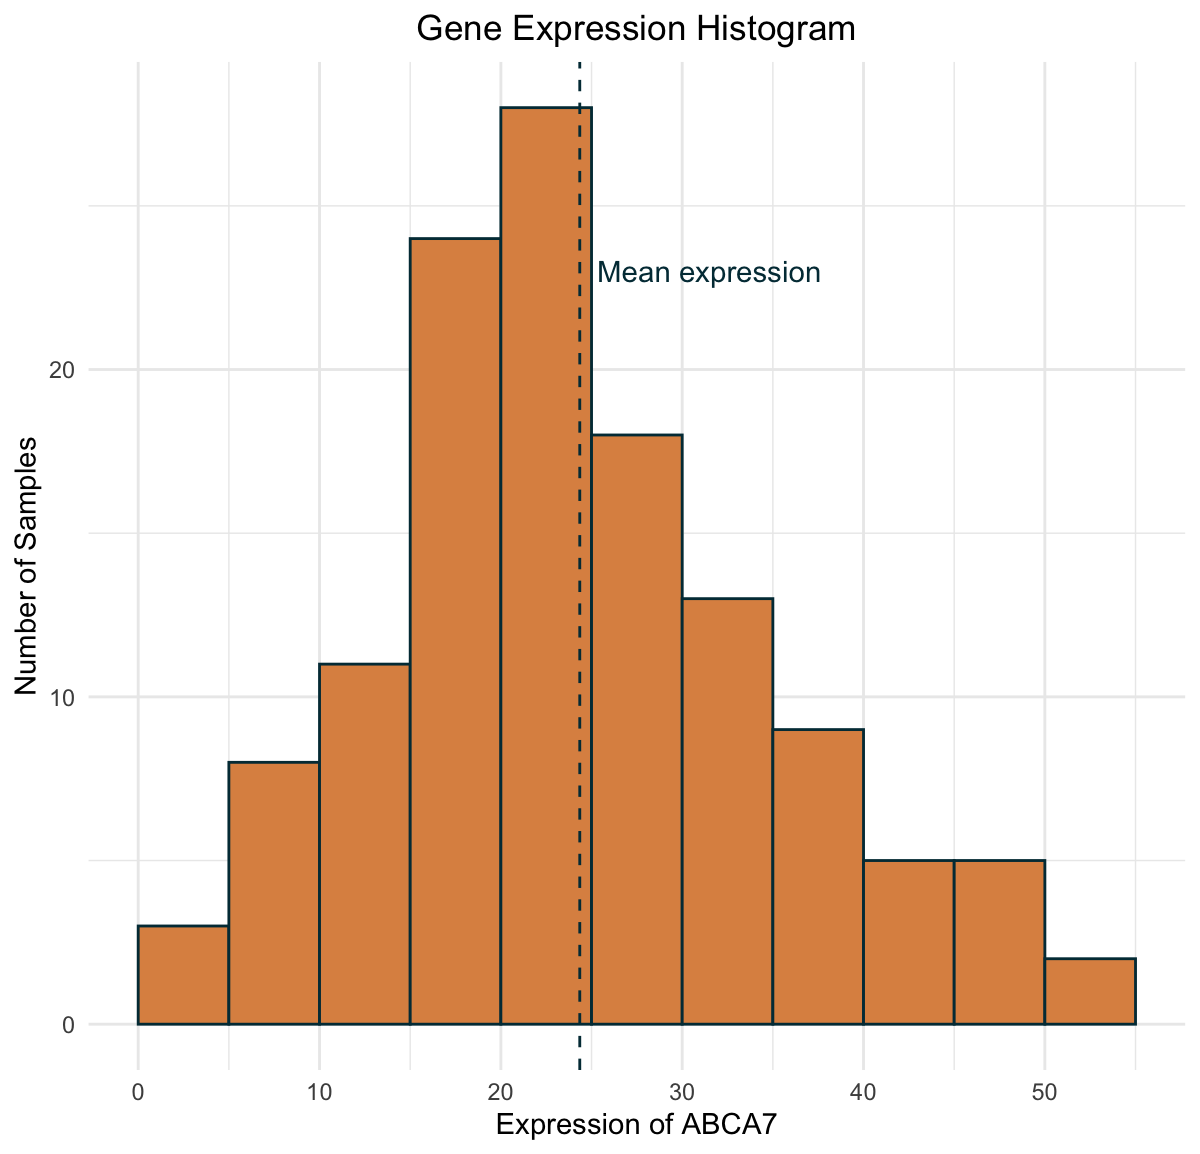
\includegraphics[width=0.75\textwidth]{plots/histogram.png}
    \caption{Expression Histogram of ABCA7}
    \label{fig: Histogram}  % Moved the label after the caption
\end{figure}

Figure \ref{fig: Histogram} displays the ABCA7 Expression Histogram. It seems to be roughly normally distributed around its mean, 24.

\begin{figure}[h!]
    \centering
    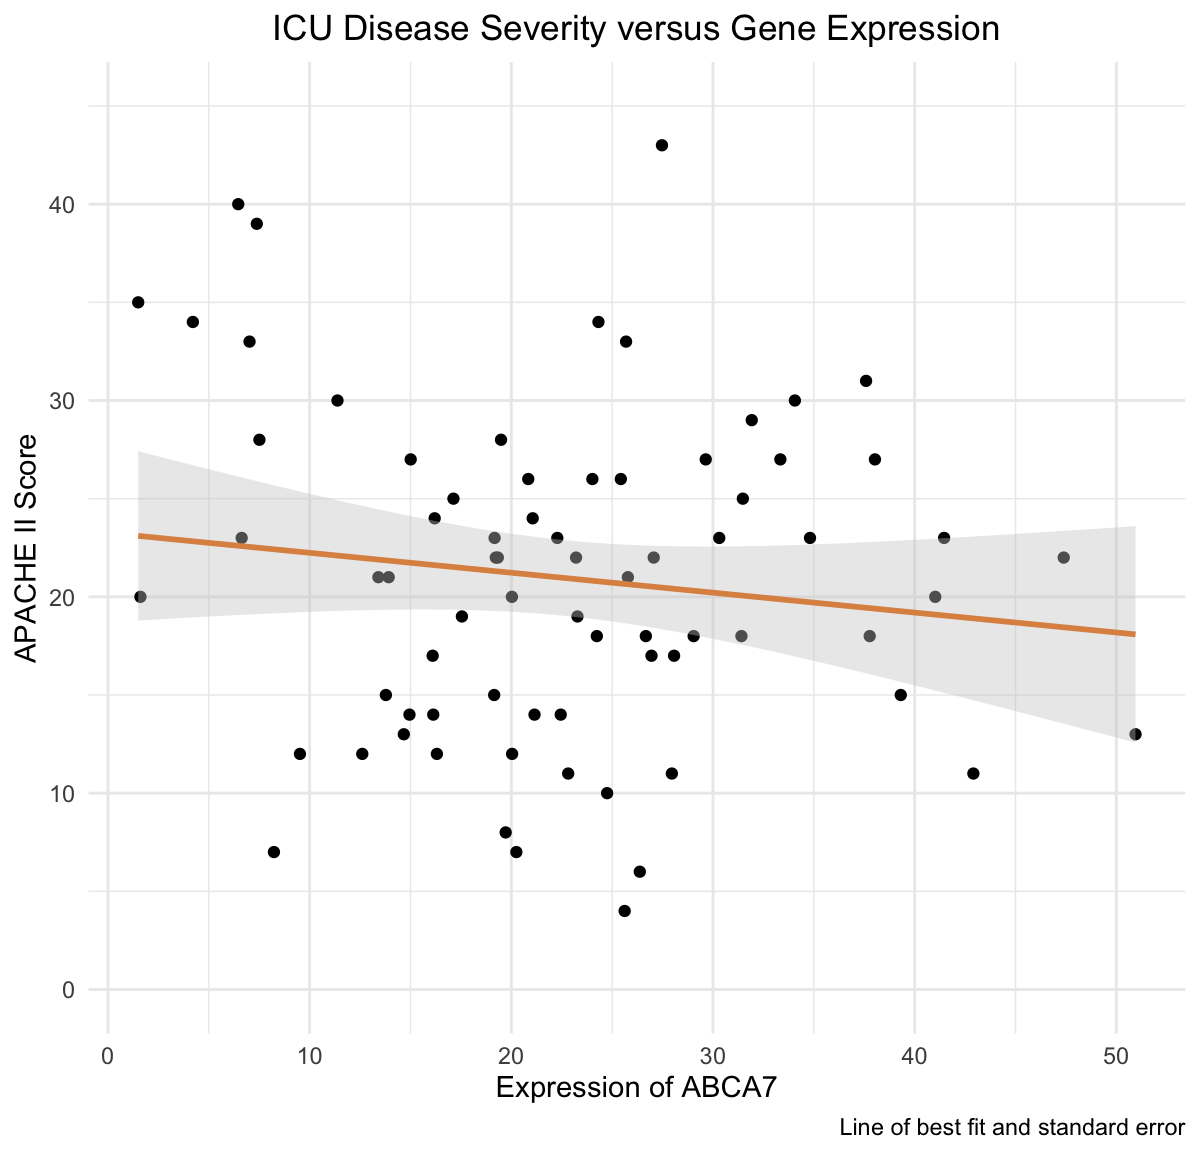
\includegraphics[width=0.6\textwidth]{plots/scatter.png}
    \caption{Scatterplot of ABCA7 vs. Apache II Score}
    \label{fig: Scatter}
\end{figure}

The Apache II score is a measure of disease severity where a higher score indicates greater medical duress. It has a negative correlation with ABCA7 expression. (Figure \ref{fig: Scatter})

\begin{figure}[h!]
    \centering
    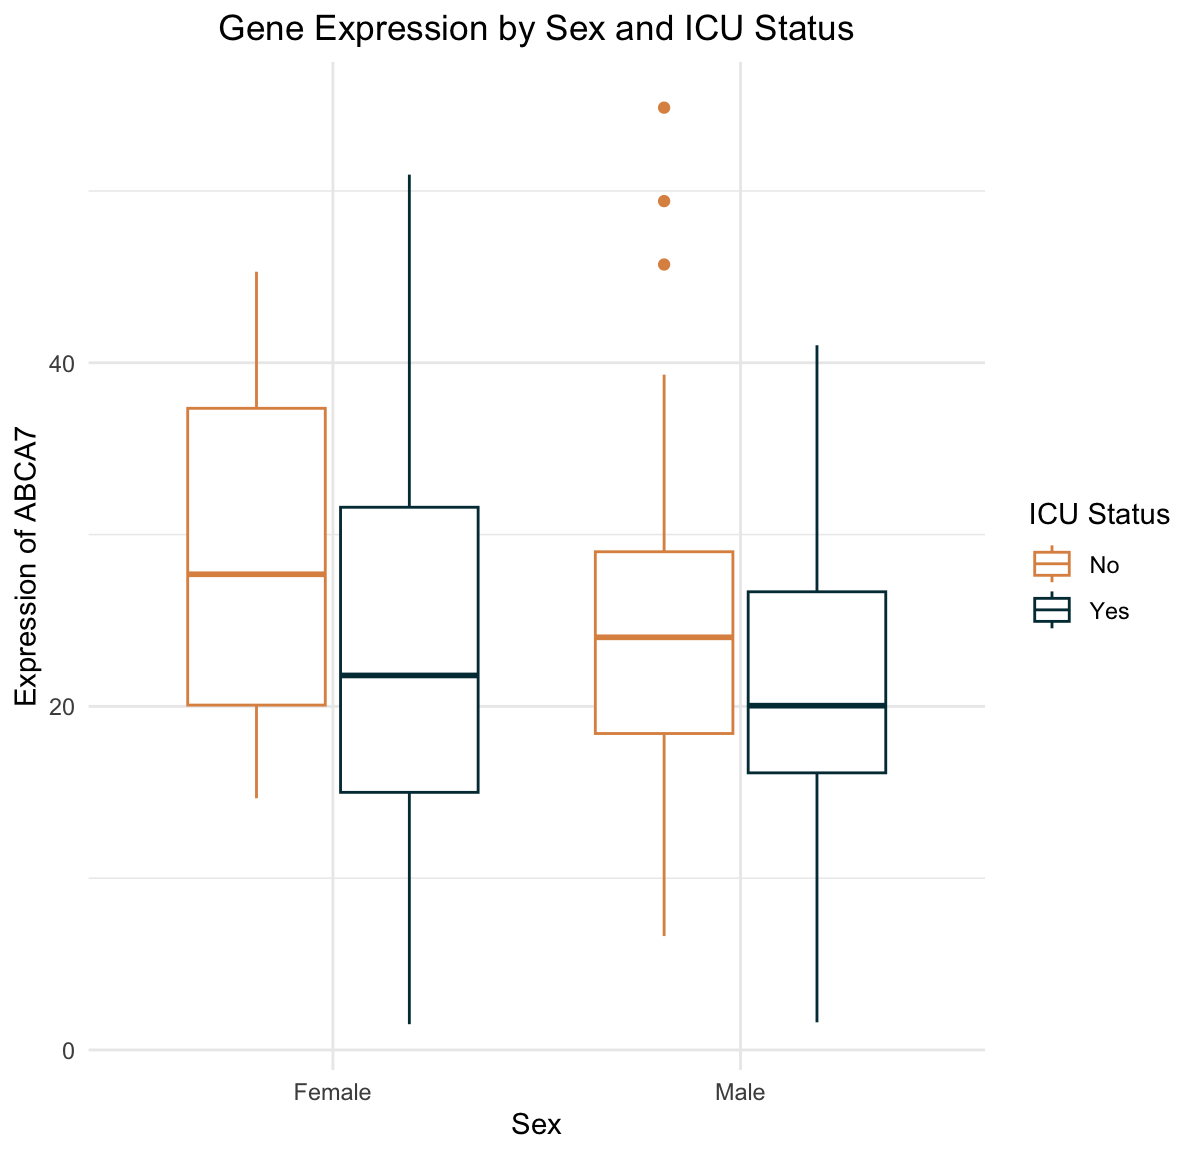
\includegraphics[width=0.6\textwidth]{plots/barplot.png}
    \caption{Boxplot of ABCA7 vs. Sex and ICU Status}
    \label{fig: Boxplot}
\end{figure}

ABCA7 expression is appears reduced generally in those in the ICU as compared to those not, and seems to be generally lower in Males versus Females. As Figure \ref{fig: Boxplot} shows, there are more high outliers in men and more low outliers in women.

\begin{figure}[h!]
    \centering
    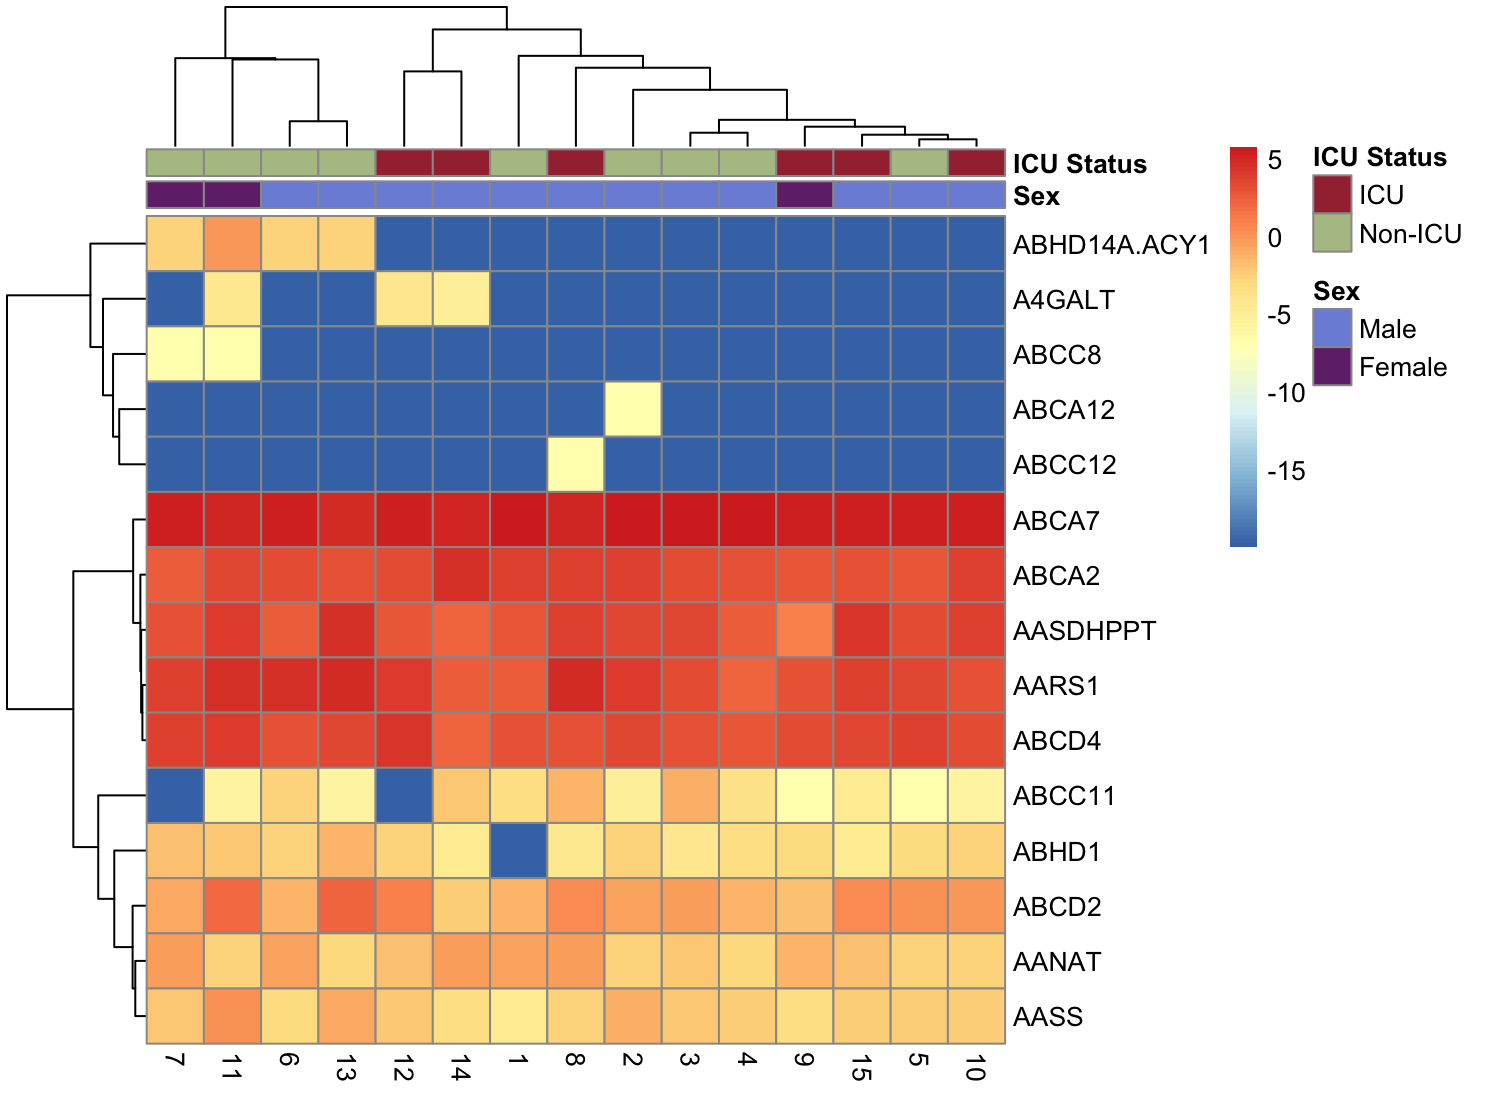
\includegraphics[width=0.75\linewidth]{plots/unscaled_heatmap.png}
    \caption{Unscaled Heatmap}
    \label{fig: Unscaled Heatmap}
\end{figure}

Without scaling, the genes appear to be highly clustered into three groups: five genes with an expression around 5, five around -5, and five around -15. Figure \ref{fig: Unscaled Heatmap} displays this very clearly, with few recognizable patterns otherwise, although most of the outlying gene expressions are associated with Non-ICU patients.

\begin{figure}[h!]
    \centering
    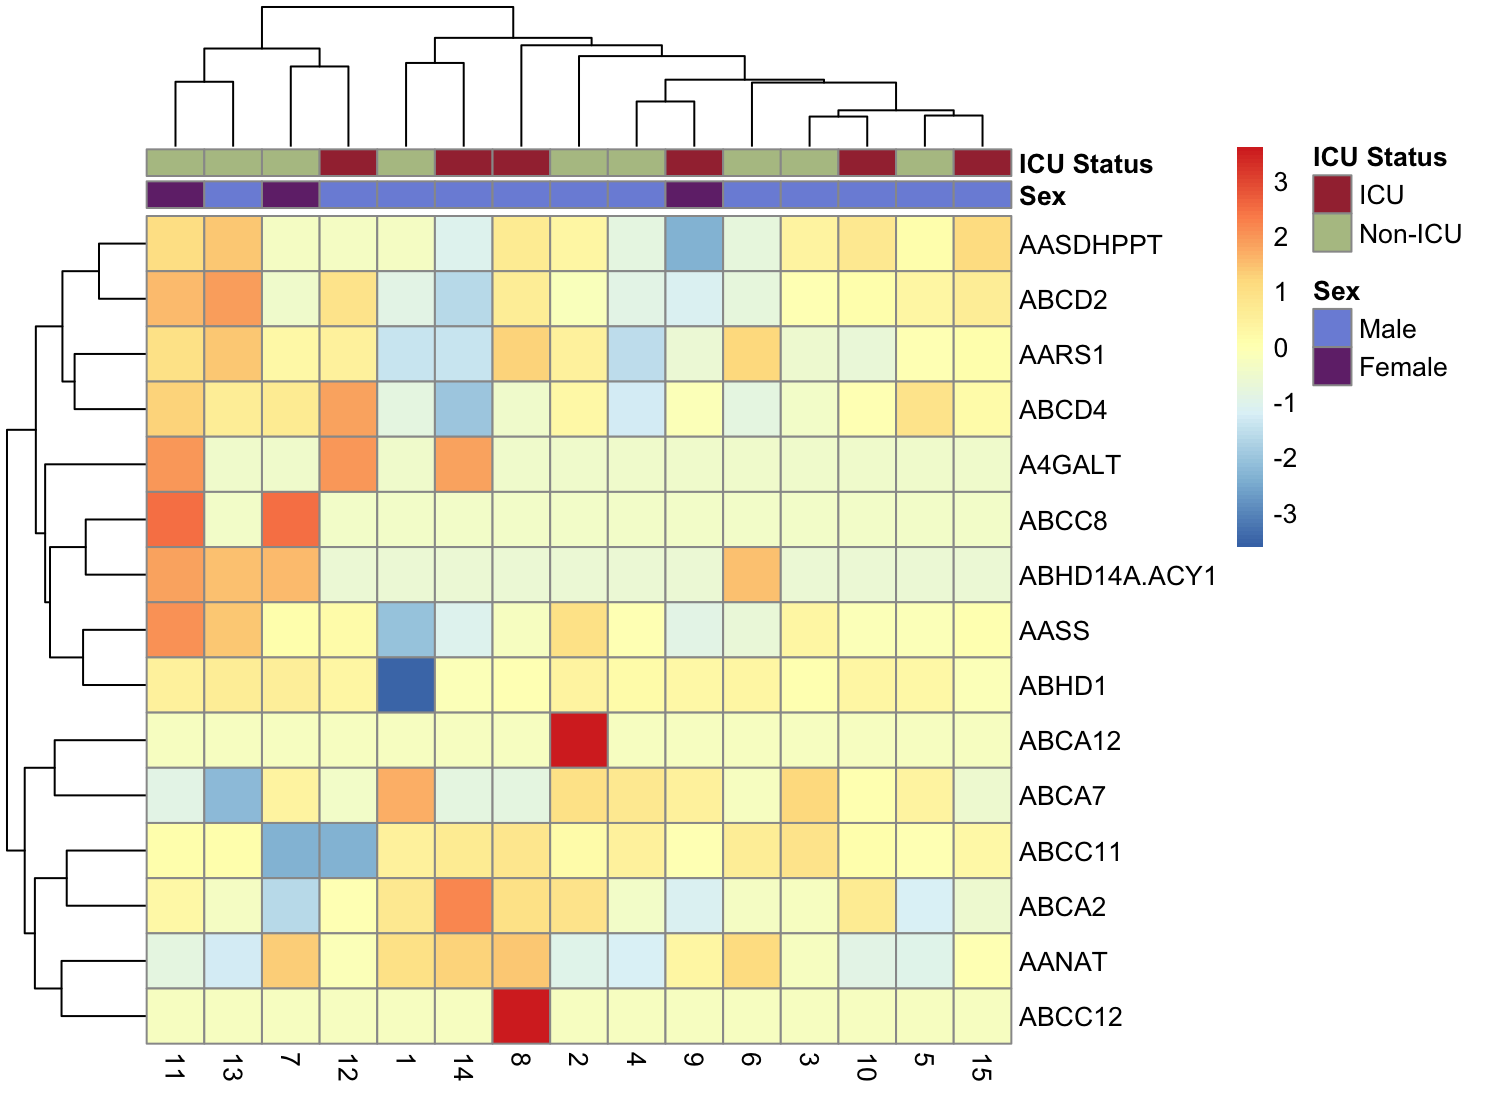
\includegraphics[width=0.75\linewidth]{plots/scaled_heatmap.png}
    \caption{Scaled Heatmap}
    \label{fig: Scaled Heatmap}
\end{figure}

The visual difference in Figure \ref{fig: Scaled Heatmap} displays the importance of scaling. Once normalized, the genes appear much less stratified and have no discernible patterns. Across Sex and ICU status there are no visible associations.

\begin{figure}[h!]
    \centering
    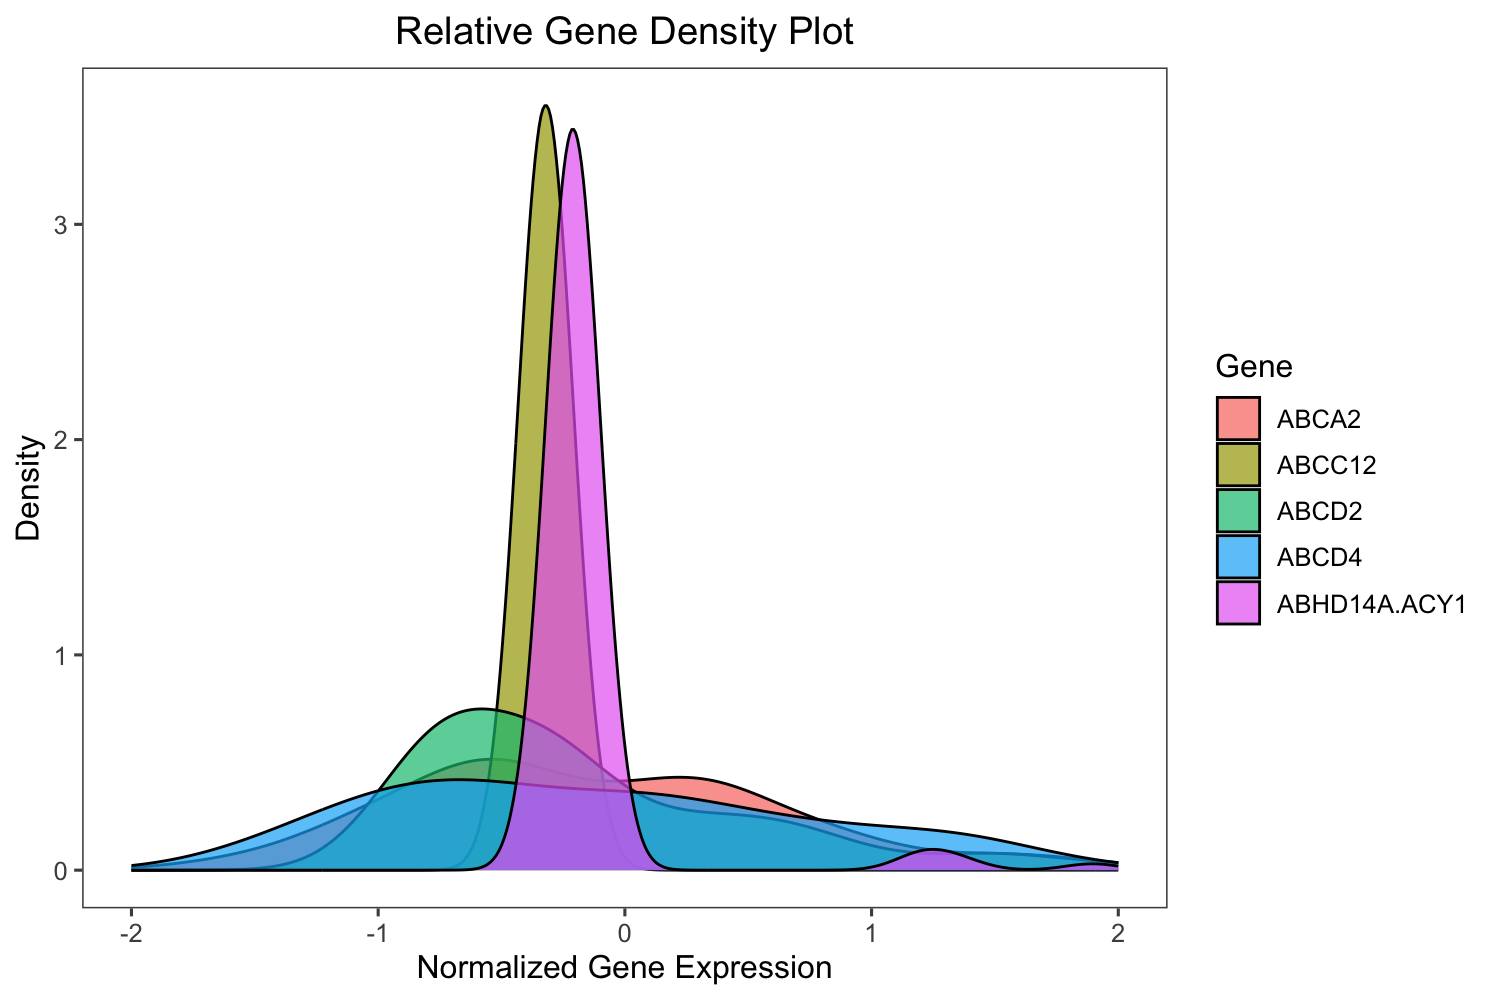
\includegraphics[width=\linewidth]{plots/density.png}
    \caption{Density Plot of Gene Subset}
    \label{fig: Density}
\end{figure}

The final plot, displayed in Figure \ref{fig: Density} is the density plot of a subset of five genes. Like the scaled heatmap, I normalize the gene expression to highlight relative differences rather than absolute. ABHD14A.ACY1 and ABC12 have narrow density bands arranged around the mean of zero while ABCD2, ABCD4, and ABCA2 have broader ranges with relatively lower density. 


\FloatBarrier
\newpage
\bibliographystyle{plain}
\bibliography{references}

\end{document}
